\documentclass[12pt]{article}
\title{Web Appendix for ``Addressing Confounding and Exposure Measurement Error Using Conditional Score Functions''}
\author{Bryan S. Blette, Peter B. Gilbert, Michael G. Hudgens}
\date{}

\usepackage{amsmath}
\usepackage{bm}
\usepackage{caption}
\usepackage[margin=1in]{geometry}
\usepackage{natbib}
\usepackage{setspace}
\doublespacing
\allowdisplaybreaks

% Table commands to match Biostatistics journal format
\newcounter{tblcap}
%\renewcommand\thetblcap{\@arabic\c@tblcap}

\newsavebox{\tabbox}
\newsavebox{\tabnotesbox}
\newlength{\tablen}
\newlength{\tabnoteslen}
%\newcommand\centerlast{%
  %\advance\leftskip by 0pt plus 1fil%
  %\advance\rightskip by 0pt plus -1fil%
   %\parfillskip0pt plus 2fil\relax}

\long\def\tblcaption#1#2{\vspace*{-5pt}
\sbox{\tabbox}{#2}
\settowidth{\tablen}{\usebox{\tabbox}}
\vskip8pt\refstepcounter{tblcap}
\centering\parbox[c]{\textwidth}{
\centerlast\noindent\mbox{\noindent\centerlast
 Appendix Table \thetblcap.}\hskip4.5pt  {\it #1}}\\[7.75pt]
\fontsize{9}{11}\selectfont \mbox{#2}}

\long\def\tblcaptionnotes#1#2#3{
\sbox{\tabbox}{#2}
\sbox{\tabnotesbox}{\fontsize{9}{11}\selectfont #2}
\settowidth{\tablen}{\usebox{\tabbox}}
\settowidth{\tabnoteslen}{\usebox{\tabnotesbox}}
\vskip8pt\refstepcounter{tblcap}
\centering\parbox[c]{\textwidth}{
\centerlast\noindent\mbox{\noindent\centerlast
 Appendix Table \thetblcap.}\hskip4.5pt  {\it #1}}\\[7.75pt]
\fontsize{9}{11}\selectfont \mbox{#2}\\[5pt]
\parbox[@{}l]{\tabnoteslen}{\fontsize{8}{10}\selectfont #3}
}

\long\def\lantblcaption#1#2{
\sbox{\tabbox}{#2}
\settowidth{\tablen}{\usebox{\tabbox}}
\vskip8pt\refstepcounter{tblcap}
\centering\parbox[c]{48pc}{
\centerlast{\noindent\mbox{\noindent\centerlast
 Table \thetblcap.}\hskip4.5pt  {\it #1}}}\\[7.75pt]
\fontsize{9}{11}\selectfont \mbox{#2}}

\long\def\lantblcaptionnotes#1#2#3{
\sbox{\tabbox}{#2}
\sbox{\tabnotesbox}{\fontsize{9}{11}\selectfont #2}
\settowidth{\tablen}{\usebox{\tabbox}}
\settowidth{\tabnoteslen}{\usebox{\tabnotesbox}}
\addtolength{\tabnoteslen}{-2.5pt}
\vskip8pt\refstepcounter{tblcap}
\centering\parbox[c]{48pc}{
\centerlast\noindent\mbox{\noindent\centerlast
 Table \thetblcap.}\hskip4.5pt  {\it #1}}\\[7.75pt]
\fontsize{9}{11}\selectfont \mbox{#2}\\[5pt]
\hspace*{4pt}\parbox[@{}l]{\tabnoteslen}{\fontsize{8}{10}\selectfont #3}
}

\def\tblhead#1{\hline\\[-9pt]#1\\\hline\\[-9.75pt]}
\def\lastline{\\\hline}

\usepackage{Sweave}
\begin{document}
\Sconcordance{concordance:Web-appendix.tex:Web-appendix.rnw:%
1 75 1 1 0 222 1}


\maketitle

\section{Web Appendix A: Large Sample Properties}

In Web Appendix A, the large sample properties of the proposed estimators discussed in section 3.6 of the paper are proven.

\subsection{G-formula CSM estimator}

\subsubsection{Large sample properties}

Consistency and asymptotic normality of the g-formula estimator are proven using standard estimating equation theory~\citep{stefanski2002}. The original CSM estimator is an M-estimator and the g-formula can be written in the form of an unbiased estimating equation. Thus, the proposed g-formula CSM estimator can be written as $\sum_{i=1}^{n} \psi_{GF-CSM}(Y_{i}, \bm{L}_{i}, \bm{A}^{*}_{i}, \Sigma_{me}, \Theta_{GF}) = 0$, where $\Theta_{GF} = (\beta_{0}, \beta^{T}_{a}, \beta^{T}_{l}, vec(\beta_{al}), \phi, E \{ Y(\bm{a}) \})$ and:
\begin{equation*}
    \psi_{GF-CSM}(Y, \bm{L}, \bm{A}^{*}, \Sigma_{me}, \Theta_{GF}) =
    \begin{bmatrix}
       \{ Y - \text{E}(Y | \bm{L}, \bm{\Delta}) \} (1, \bm{L}, \bm{\Delta}, \bm{L} \otimes \bm{\Delta})^{T} \\
        \phi - \{ Y - \text{E}(Y | \bm{L}, \bm{\Delta}) \}^{2} / \{ \text{Var}(Y | \bm{L}, \bm{\Delta}) / \phi \} \\
        g^{-1}(\beta_{0} + \bm{a}\beta_{a} + \bm{L}\beta_{l} +
        \bm{a}\beta_{al}\bm{L}^{T}) - E \{ Y(\bm{a}) \}
    \end{bmatrix}
\end{equation*}

The parameter of interest $E \{ Y(\bm{a}) \}$ is in the last estimating equation of the stack, and the proof relies on (i) the usual g-formula proof based on the causal assumptions made in Section 2 of the paper and (ii) that the CSM estimator $\hat{E}(Y | \bm{A} = \bm{a}, \bm{L})$ was previously shown to be consistent~\citep{carroll2006}:

\begin{align*}
E[g^{-1}(\beta_{0} + \bm{a}\beta_{a} + \bm{L}\beta_{l} +
        \bm{a}\beta_{al}\bm{L}^{T}) - E \{ Y(\bm{a}) \}] &= E \{ g^{-1}(\beta_{0} + \bm{a}\beta_{a} + \bm{L}\beta_{l} +
        \bm{a}\beta_{al}\bm{L}^{T}) \} - E \{ Y(\bm{a}) \} \\
&= E \{ \hat{E}(Y | \bm{A} = \bm{a}, \bm{L}) \} - E[E \{ Y(\bm{a}) | \bm{L} \}] \\
&= E \{ E(Y | \bm{A} = \bm{a}, \bm{L}) \} - E[E \{ Y(\bm{a}) | \bm{A} = \bm{a}, \bm{L} \}] \\
&= E \{ E(Y | \bm{A} = \bm{a}, \bm{L}) \} - E\{ E(Y | \bm{A} = \bm{a}, \bm{L})\} \\
&=0
\end{align*}

So the estimating function for the parameter $E \{ Y(\bm{a}) \}$ is unbiased. Denote $\hat{\Theta}_{GF}$ as the solution to $\sum_{i=1}^{n} \psi_{GF-CSM}(Y_{i}, \bm{L}_{i}, \bm{A}^{*}_{i}, \Sigma_{me}, \hat{\Theta}_{GF}) = 0$. Then by the proof above $\sqrt{n}(\hat{\Theta}_{GF} - \Theta_{GF}) \sim N(\textbf{0}, A^{-1}B(A^{-1})^{T})$ where $A$ and $B$ are consistently estimated by

\begin{equation*}
\hat{A} = \frac{1}{n} \sum_{i=1}^{n} \frac{d}{d\Theta_{GF}^{T}} \psi_{GF-CSM}(Y_{i}, \bm{L}_{i}, \bm{A}^{*}_{i}, \Sigma_{me}, \hat{\Theta}_{GF})
\end{equation*}
\begin{equation*}
\hat{B} = \frac{1}{n} \sum_{i=1}^{n} \psi_{GF-CSM}(Y_{i}, \bm{L}_{i}, \bm{A}^{*}_{i}, \Sigma_{me}, \hat{\Theta}_{GF}) \psi^{T}_{GF-CSM}(Y_{i}, \bm{L}_{i}, \bm{A}^{*}_{i}, \Sigma_{me}, \hat{\Theta}_{GF})
\end{equation*}
In the R code implementing the methods, this sandwich variance estimation is accomplished using the R package geex~\citep{saul2017}.

\subsubsection{Relationship to classical causal estimators}

It has been noted (see \citet{carroll2006}) that the CSM estimating equations reduce to the score equations for a GLM when the measurement error covariance matrix $\Sigma_{me} = 0_{m \times m}$. Thus under no measurement error, the procedure described above reduces to a stack of estimating equations corresponding to the common practice of performing the g-formula while specifying a GLM for the outcome regression, making it a special case of the proposed estimator.

\subsection{IPW CSM estimator}

\subsubsection{Large sample properties}

Consistency and asymptotic normality of the IPW CSM estimator are proven as above, using M-estimator theory. The partial M-estimator~\citep{stefanski2002} corresponding to the parameters of interest is $\sum_{i=1}^{n} \psi(Y_{i}, \bm{Z}_{i}, \bm{L}_{i}, \bm{A}^{*}_{i}, \Theta_{IPW}) = \sum_{i=1}^{n} SW_{i}(Y_{i} - E[Y_{i} | \bm{\Delta}_{i}])\bm{\Delta}_{i}^{T} = 0$. It suffices to show that the expectation of the estimating function $\psi(Y, \bm{Z}, \bm{L}, \bm{A}^{*}, \Theta_{IPW})$ is equal to 0. Although $\bm{\Delta} = (\Delta_{1}, ..., \Delta_{m})$ is a vector of length $m$, the estimator form is the same for each row of the estimating equation stack and without loss of generality, the estimating function is proven to be unbiased for $SW(Y - E[Y | \bm{\Delta}])\Delta_{k}$ for an arbitrary $1 \leq k \leq m$.

First consider the estimator as written, where it is weighted by the true propensity weights which aren't typically known in practice. Let $SW = \frac{h(\bm{A})}{f(\bm{A} | \bm{L})}$ such that the numerator is any function of $\bm{A}$ and the denominator is a conditional density of exposures given confounders. Furthermore, suppose that the denominator density equals the true conditional density, denoted $f(\bm{A} | \bm{L}) = f_{0}(\bm{A} | \bm{L})$. Let $E_{0}$ notation refer to taking the expectation under the true causal parameter vector from the MSM, which is nested within $E(Y | \bm{\Delta})$. In a slight abuse of notation, let $\Delta_{k}$ be the random variable corresponding to the $k^{th}$ element of the random vector $\bm{\Delta}$, rather than the vector $\bm{\Delta}$ for individual $k$ which is instead notated as bold $\bm{\Delta}_{k}$ in the manuscript.

\begin{align*}
E_{0} \bigg[\frac{h(\bm{A})}{f_{0}(\bm{A} | \bm{L})} \{ Y - E(Y | \bm{\Delta})\} \Delta_{k} \bigg] &= E_{0} \left( E \bigg[\frac{h(\bm{A})}{f_{0}(\bm{A} | \bm{L})} \{ Y^{\bm{A}} - E(Y^{\bm{A}} | \bm{\Delta}) \} \Delta_{k} | \bm{L} \bigg] \right) \\
&= E_{0} \left [ \int_{\bm{a}} \frac{h(\bm{a})}{f_{0}(\bm{a} | \bm{L})}\{ Y^{\bm{a}} - E(Y^{\bm{a}} | \bm{\Delta}) \} \Delta_{k} f_{0}(\bm{a} | \bm{L}) d\mu (\bm{a}) \right ] \\
&= E_{0} \left \{ \int_{\bm{a}} h(\bm{a})(Y^{\bm{a}} - E[Y^{\bm{a}} | \bm{\Delta}])\Delta_{k} d\mu (\bm{a}) \right \} \\
&= \int_{\bm{a}} E_{0} \left \{ h(\bm{a})(Y^{\bm{a}} - E[Y^{\bm{a}} | \bm{\Delta}])\Delta_{k} \right \} d\mu (\bm{a}) \\
&= \int_{\bm{a}} E_{0} \left \{ E \bigg[ h(\bm{a})(Y^{\bm{a}} - E[Y^{\bm{a}} | \bm{\Delta}])\Delta_{k} | \bm{\Delta} \bigg] \right \} d\mu (\bm{a}) \\
&= \int_{\bm{a}} E_{0} \left \{ h(\bm{a})\Delta_{k} E \bigg[ (Y^{\bm{a}} - E[Y^{\bm{a}} | \bm{\Delta}]) | \bm{\Delta} \bigg] \right \} d\mu (\bm{a}) \\
&= \int_{\bm{a}} E_{0} \left \{ h(\bm{a})\Delta_{k} ( E[Y^{\bm{a}} | \bm{\Delta}] - E[Y^{\bm{a}} | \bm{\Delta}] ) \right \} d\mu (\bm{a}) \\
&= 0
\end{align*}
where $d\mu (\bm{a})$ is defined as the Lebesgue measure. The first equality uses causal consistency, the second equality uses conditional exchangeability, and positivity is needed for the integral to be well-defined. Thus the estimator is consistent and asymptotically normal by standard M-estimator theory. The asymptotic variance is given by the usual sandwich estimator as described in the previous section.

From here there are two jumps to the corresponding estimator when weights are estimated. The first is that one needs to estimate the treatment weights from some kind of model, even if no treatments were mismeasured. This substitution is well known to result in a consistent estimator as long as the propensity score model is correctly specified, because then this estimator will equal the estimator described above plus an $o_{p}(1)$ term. The second jump was alluded to in Section 3.3 of the paper, that one can use weights estimated from a propensity model that is fit using the mismeasured exposures. This will not necessarily affect the consistency of the estimator. For example, suppose the exposures are independent given $\bm{L}$ and that each exposure has a linear relationship with the confounders, i.e., with simplified scalar notation, $A = \bm{L} \alpha + \epsilon_{ps}$. Then under additive measurement error, each mismeasured observed exposure also has a linear relationship with the confounders given by: $A^{*} = \bm{L} \alpha + \epsilon_{ps} + \epsilon_{me}$. So if linear propensity models are fit using the mismeasured exposures (noting that $\bm{A}^{*}$ is a collider on the only path connecting $\epsilon_{me}$ and $\bm{L}$), one would still get consistent estimates of the propensity model parameters $\alpha$ (and subsequently the weights), albeit with more variability. Therefore the proposed estimator would still be consistent. When exposures have non-linear, complex relationships with confounders, consistency may not be guaranteed, but previous explorations of this topic suggest that the measurement error will likely only introduce mild issues~\citep{carroll2006}.

\subsubsection{Relationship to classical causal estimators}

Note that when the measurement error covariance matrix $\Sigma_{me} = \textbf{0}_{m \times m}$, the sufficient statistic $\bm{\Delta}$ reduces to the observed exposure vector. Then the IPW estimator reduces to the form $\sum_{i=1}^{n} \psi(Y_{i}, \bm{L}_{i}, \bm{A}^{*}_{i}, \Theta_{IPW}) = 0$ where:

\begin{equation*}
    \psi(Y, \bm{L}, \bm{A}^{*}, \Theta_{IPW}) =
    \begin{bmatrix}
       SW\{ Y - E(Y | \bm{A}^{*}) \} (1, \bm{A}^{*})^{T} \\
       SW \left [ \phi - \frac{ \{Y - E(Y | \bm{A}^{*}) \}^{2}}{Var(Y | \bm{A}^{*}) / \phi} \right ]
    \end{bmatrix}
\end{equation*}
This is exactly the score function vector for a GLM weighted by $SW$. Thus, an IPW estimator fit using a weighted GLM for outcome $Y$ is a special case of the proposed IPW CSM estimator where there is no measurement error present.

\subsection{DR CSM Estimator}

\subsubsection{Large Sample Properties}

Once again, consistency and asymptotic normality of the proposed estimator is proven using M-estimator theory. This estimator is a solution to the estimating equation \newline $\sum_{i=1}^{n} \psi_{DR-CSM}(Y_{i}, \bm{L}_{i}, \bm{A}_{i}^{*}, \Sigma_{me}, \Theta_{DR}) = 0$, where $\Theta_{DR} = \Theta_{GF}$ and
\begin{equation*}
    \psi_{DR-CSM}(Y, \bm{L}, \bm{A}^{*}, \Sigma_{me}, \Theta_{DR}) =
    \begin{bmatrix}
       SW\{ Y - \text{E}(Y | \bm{L}, \bm{\Delta}) \} (1, \bm{L}, \bm{\Delta}, \bm{L} \otimes \bm{\Delta})^{T} \\
        SW[\phi - \{ Y - \text{E}(Y | \bm{L}, \bm{\Delta}) \}^{2} / \{ \text{Var}(Y | \bm{L}, \bm{\Delta}) / \phi \}] \\
        g^{-1}(\beta_{0} + \bm{a}^{*}\beta_{a} + \bm{l}\beta_{l} +
        \bm{a}^{*}\beta_{al}\bm{l}^{T}) - E \{ Y(\bm{a}) \}
    \end{bmatrix}
\end{equation*}

First, suppose that the propensity score models are correctly specified. This effectively means that we are fitting the outcome regression in a pseudo-population where the effect of treatment on the outcome is no longer confounded. This means that integrating out $\bm{L}$ in the standardization step will have no effect, and the DR CSM estimator will be asymptotically equivalent to the IPW estimator, which was previously shown to be consistent and asymptotically normal when the propensity models are correctly specified.

Now, suppose that the outcome regression is correctly specified. Then the proof follows the same form as the g-formula CSM proof since the outcome predictions from the IP-weighted CSM model converge in expectation to outcome predictions from the non-weighted CSM model regardless of whether the propensity model is correctly specified. However, the $\hat{\beta}$ estimated by the DR CSM estimator when the propensity model is mis-specified may be a particularly inefficient estimator of the true $\beta$ outcome model parameters. \citet{robins2007} considered this a notable weakness of this type of DR estimator, but also concluded that this DR estimator form is stronger than other described DR forms when weights are highly variable (which is extremely common in the continuous exposure setting \citet{naimi2014}).

\subsubsection{Relationship to classical causal estimators}

Once again, under no measurement error the CSM equations reduce to the score equations of a GLM. Thus the proposed DR CSM estimator will reduce to the DR estimator described in \citet{hirano2001} where the specified outcome regression is a GLM.

\subsection{Uniqueness of EE solutions}

Each of the proofs above relies on there being a unique solution to each set of estimating equations. It has been noted in prior work~\citep{stefanski1987} that similar conditional score equations do not always have unique solutions, but that multiple solutions are very rare in practice. In the various simulations of this paper, multiple solutions or estimator divergence were encountered with similar rarity, at most 1 or 2 times per 2000 simulations, unless considering extreme data generating mechanisms. Thus, the estimators should have good behavior in general, but practitioners should be aware of rare instances of multiple solutions, unusual estimates, and/or root-solving algorithm divergence errors.

\section{Web Appendix B: Accounting for Two-Phase Sampling}

Many studies (including the HVTN 505 trial) use a two-phase sampling design. Such a design is particularly useful when the primary exposure(s) and outcome are easy to measure, but exposures and covariates of secondary interest are expensive or difficult to measure. Because each of the proposed methods above belongs to the estimating equation framework, it is straightforward to incorporate previously described methods for causal inference from studies with two-phase sampling. In this section, one such approach is demonstrated using a simulation study. In particular, for this simulation and the application section analysis, the simple IPW method described in \citet{wang2009} is implemented, but the DR approaches from the same paper or from \citet{rose2011} could also be explored to account for two-phase sampling within the proposed methods.

The simple IPW method is implemented by weighting each of the proposed estimating equations by the inverse probability of selection for the second-phase of the study (multiplying treatment weights by sampling weights for the IPW-CSM and DR-CSM estimators) and restricting the analysis to those selected. This works well for the subset of the HVTN 505 trial that is the focus of Section 5 of the paper, but may be inadequate when analyzing exposures measured in a sub-sample in conjunction with exposures measured in the full sample.

\subsection{Two-phase sampling simulations}

The structure of the first simulation study described in Section 4 of the paper is replicated, but under a two-phase sampling design. In particular, a case-cohort design is used where the exposure is measured for a random sub-cohort as well as for every case. This is done for a sample size of $n=2000$ under three scenarios, with sub-cohorts of size $5\%$, $10\%$ and $25\%$. The results of 2000 simulation runs are presented in Appendix Figure 1 and Appendix Table 1, with Bias, ASE, ESE, and Coverage defined as in Table 1 of the paper.

\begin{figure}
\centering
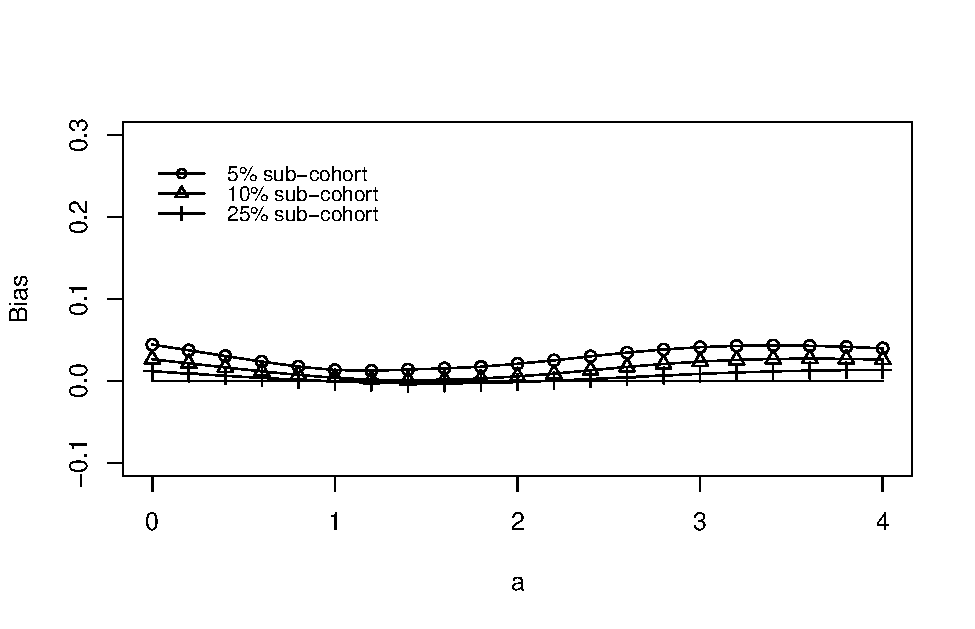
\includegraphics[width=6in]{app_fig1.pdf}
\caption{Estimated dose-response curve bias for the DR CSM method compared across three sub-cohort sizes. Bias refers to the average bias across 2,000 simulated data sets for each method evaluated at each point on the horizontal axis $a = (0, 0.2, 0.4, ..., 4)$.}
\end{figure}

The methods seem to perform well as they did in the full-sampling simulation provided in the paper, although there is some bias and under-coverage when the sub-cohorts are smaller, likely due to a low effective sample size. In addition, the estimators failed to converge in some of the small sub-cohort settings. However, the DR CSM estimator with sampling weights converged in all analyses presented in Section 5 of the paper.

\begin{table}[h]
\tblcaption{Simulation study for case-cohort design}
{\tabcolsep=6.25pt
\begin{tabular}{@{}lcrrrr@{}}
\tblhead{Sub-cohort Size & Bias & ASE & ESE & Coverage & Percent failed to converge}
5\% & 4.1 & 8.7 & 7.1 & 84\% & 6\% \\
10\% & 2.4 & 6.3 & 5.6 & 90\% & 2\% \\
25\% & 0.9 & 4.1 & 3.9 & 94\% & 0\%
\lastline
\end{tabular}}
\end{table}

\section{Web Appendix C: Additional Simulations}

In this section, the methods are studied under two assumption violations: (i) when positivity doesn't hold and (ii) when measurement error doesn't follow a classical additive model.

\subsection{Under positivity violation}

To evaluate the proposed g-formula CSM method under positivity violation, the general structure of the first simulation study from Section 4 of the paper is replicated almost exactly. A moderate positivity violation is created by changing how the treatment $A_{1}$ is generated from $\mathcal{N}(2 + 0.3L_{1} - 0.5L_{2}, 0.6)$ to $\mathcal{N}(2 + 0.3L_{1} - 0.5L_{2}, 0.35)$. This breaks the phenomenon of mostly overlapping treatment values experienced by simulated subjects with different covariate values, although in a technical sense is not a structural violation of positivity since the distributions would have the same support given infinite sample size. The results of the simulation study are presented in Appendix Figure 2 and Appendix Table 3, following the same format as Table 1 and Figure 2 in the paper.

\begin{figure}
\centering
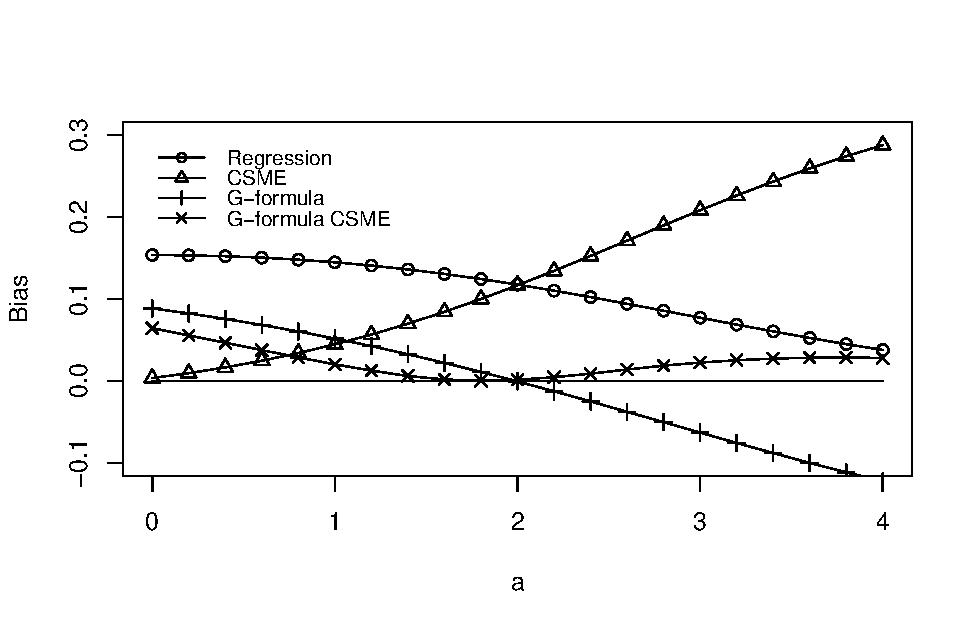
\includegraphics[width=6in]{app_fig2.pdf}
\caption{Estimated dose-response curve bias for each of the four methods. Bias refers to the average bias across 2,000 simulated data sets for each method evaluated at each point on the horizontal axis $a = (0, 0.2, 0.4, ..., 4)$.}
\end{figure}

The results overall look similar to that in Table 1 of the paper. There is some bias and undercoverage for the proposed g-formula CSM methods, but the proposed method still generally performs better than the comparator methods in this scenario. Performance is weaker at the extremes of the exposure support, which is expected given that there is very little data at the extremes with the new data generating mechanism and not fully due to the positivity violation. A reasonable range to evaluate the methods would be from 0.5 to 3.5 in these simulations.

Positivity violations become more likely with more treatment variables and with treatment variables that are continuous or take on many values. In these settings positivity should receive just as much scrutiny as the conditional exchangeability assumption. If positivity is implausible, it may be possible to define an estimator in our setting similar to that described in \citet{neugebauer2005} which was robust to their analogous "experimental treatment assumption".

\begin{table}[h]
\tblcaption{Simulation study under positivity violation}
%\caption*{Appendix Table 1: Simulation study under positivity violation}
{\tabcolsep=4.25pt
\begin{tabular}{@{}lrrrr@{}}
\tblhead{Estimator & Bias & ASE & ESE & Coverage}
Regression & -69.8 & 21.5 & 21.8 & 11\% \\
CSM & -17.0 & 80.3 & 68.5 & 95\% \\
G-formula & -6.3 & 3.0 & 3.0 & 44\% \\
G-formula CSM & 2.2 & 9.3 & 9.1 & 92\%
\lastline
\end{tabular}}
\end{table}

\subsection{Under non-additive measurement error}

Next the proposed methods are evaluated when treatment measurement error does not follow the classical additive model. In particular, the second simulation study from Section 4 of the paper is replicated, but the simulation of mismeasured treatment $A^{*}_{3}$ is changed such that it follows a multiplicative error model simulated as $A_{3}^{*} = A_{3} \epsilon_{me_{1}}$ where $\epsilon_{me_{1}} \sim \mathcal{N}(1, 0.1)$. The methods are still performed assuming additive measurement error with known measurement error covariance as specified in section 4 of the paper, and the $A^{*}_{3}$ distribution under this additive ME assumption is similar to the distribution under the true multiplicative ME generative model. The results are presented in Appendix Table 4. The proposed IPW CSM method continued to perform well for treatments $A_{1}$ and $A_{2}$ for which the assumptions hold, but exhibited strong bias for the $A_{3}$ effect. Practitioners of the proposed methods should be cautious that if classical additive measurement error models do not hold for their exposures, they may get worse results than even standard regression models.

\begin{table}[h]
\tblcaption{Simulation study under non-additive measurement error}
{\tabcolsep=4.25pt
\begin{tabular}{@{}lrrrrrrrrrrrr@{}}
\tblhead{ & $\psi_{1}$ &&&& $\psi_{2}$ &&&& $\psi_{3}$ &&& \\
Estimator & Bias & ASE & ESE & Coverage & Bias & ASE & ESE & Coverage & Bias & ASE & ESE & Coverage}
Regression & 4.9 & 14.0 & 13.3 & 93\% & 10.3 & 28.0 & 27.7 & 93\% & 1.9 & 15.8 & 15.4 & 94\% \\
CSM & 21.7 & 20.0 & 19.3 & 82\% & 8.7 & 29.4 & 28.4 & 93\% & -35.0 & 33.5 & 32.7 & 86\% \\
IPW & -9.9 & 9.1 & 9.0 & 79\% & 0.0 & 20.0 & 19.7 & 94\% & 4.7 & 15.9 & 15.5 & 93\% \\
IPW CSM & 0.6 & 13.0 & 12.7 & 95\% & -0.9 & 20.4 & 20.1 & 95\% & -29.0 & 33.0 & 32.0 & 88\%
\lastline
\end{tabular}}
\end{table}

\section{Web Appendix D: More complex model specifications for the IPW CSM estimator}

The proposed IPW CSM estimator assumes a linear marginal structural model form. While this is helpful to match the conditional score framework described in Section 3.1, it is too restrictive for some potential applications. To this end we note that transformations of elements of $\bm{A}$ and interactions thereof can be included in the MSM specification as long as they are either assumed to be correctly measured or assumed to follow a classical additive measurement error model. For example, if a transformation of an exposure is assumed to follow a multiplicative measurement error model then that variable cannot be included in the MSM. However, if the variable is strictly positive, then its log transform would follow an additive measurement error model and can be included in the model. In general, transformations of correctly measured exposures can be included in the MSM specification without restriction.

Finally, while conditional score functions are somewhat limited in scope in terms of model specification, the related method of corrected score functions has been extended to problems of additive but non-normal measurement error~\citep{buzas1996} and to non-additive measurement models in certain cases (\citealp{nakamura1990}; \citealp*{li2004}). Describing how to use such corrected score functions to estimate causal parameters could be the focus of future work in this area.

\bibliographystyle{biom}
\bibliography{refs}

\end{document}
